\documentclass[letterpaper]{sig-alternate-10pt}
\usepackage{url,xspace,subfigure,multirow}
\usepackage{color,cite,graphicx}


%%% PG2013:: bunch of macros you can ignore them for now 
\def\full{0}        % set 1 for a full tech report version
                    % set 0 for submission version
\def\shownotes{0}   % set 1 for version with author notes
                    % set 0 for no notes
\def\anon{0}        % set 1 to anonymize
                    % set 0 for acks and author names

\def\showedits{0} %set for 1 to turn edits red, 0 for them to become black.

\newcommand{\namedref}[2]{#1~\ref{#2}}
\newcommand{\tableref}[1]{\namedref{Table}{#1}}
\newcommand{\sectionref}[1]{$\S$\ref{#1}}
\newcommand{\appendixref}[1]{\namedref{Appendix}{#1}}
\newcommand{\theoremref}[1]{\namedref{Theorem}{#1}}
\newcommand{\remarkref}[1]{\namedref{Remark}{#1}}
\newcommand{\definitionref}[1]{\namedref{Definition}{#1}}
\newcommand{\figureref}[1]{\namedref{Figure}{#1}}
\newcommand{\lemmaref}[1]{\namedref{Lemma}{#1}}
\newcommand{\claimref}[1]{\namedref{Claim}{#1}}
\newcommand{\propositionref}[1]{\namedref{Proposition}{#1}}
\newcommand{\constructionref}[1]{\namedref{Construction}{#1}}
\newcommand{\corollaryref}[1]{\namedref{Corollary}{#1}}
\newcommand{\equationref}[1]{\namedref{Equation}{#1}}
%
\newtheorem{theorem}{Theorem}[section]
\newtheorem{definition}[theorem]{Definition}
\newtheorem{lemma}[theorem]{Lemma}
\newtheorem{claim}[theorem]{Claim}
\newtheorem{proposition}[theorem]{Proposition}
\newtheorem{obs}[theorem]{Observation}
%

%%%%%%%  Author Notes %%%%%%%
%
\ifnum\shownotes=1
\newcommand{\authnote}[2]{{ $\ll$\textsf{\footnotesize #1 notes: #2}$\gg$}}
\else
\newcommand{\authnote}[2]{}
\fi
\newcommand{\Dnote}[1]{{\authnote{Dave}{#1}}}
\newcommand{\Anote}[1]{{\authnote{Abbas}{#1}}}
\newcommand{\Pnote}[1]{{\authnote{Phillipa}{#1}}}

%edits
\ifnum\showedits=1
\newcommand{\edit}[1]{\textcolor{red}{#1}}

\else
\newcommand{\edit}[1]{\textcolor{black}{#1}}
\fi

%%%%%%%%%%%%%%%%%%%%%%%%%%%%%%%%%

\providecommand{\vs}{vs. }
\providecommand{\ie}{\emph{i.e.,} }
\providecommand{\eg}{\emph{e.g.,} }
\providecommand{\cf}{\emph{cf.,} }
\providecommand{\resp}{\emph{resp.,} }
\providecommand{\etal}{\emph{et al. }}   %Removed trailing space here; usually want non-breaking space with following reference
\providecommand{\etc}{\emph{etc.}}      % No trailing space here either
\providecommand{\mypara}[1]{\smallskip\noindent\emph{#1} }
\providecommand{\myparab}[1]{\smallskip\noindent\textbf{#1} }
\providecommand{\myparasc}[1]{\smallskip\noindent\textsc{#1} }
\providecommand{\para}{\smallskip\noindent}



\title{Traffic Differentiation on Cellular Data Networks}
%\subtitle{subtitle (optional)}



\ifnum\anon=0
\author{Arash Molavi Kakhki, Abbas Razaghpanah, Phillipa Gill, Alan Mislove, Dave Choffnes}
\else
\author{[Paper \#, X pages]}
\fi


\begin{document}
%% COPYRIGHT STUFF
%\iffalse
%\conferenceinfo{SIGCOMM'11,} {August 15-19, 2011, Toronto, Ontario, Canada.}
%\CopyrightYear{2011}
%\crdata{978-1-4503-0797-0/11/08}
%\fi

\clubpenalty=10000
\widowpenalty = 10000

\maketitle

\section*{Abstract}
{\it
As wireless providers offer faster and more widely available cellular data to their customers, more mobile applications emerge that utilize this to add more services to the mobile platform or just simply improve on the quality of existing ones. It is not clear how traffic from said services is treated while traversing boundaries of these networks.

The goal of this research is to detect traffic differentiation in cellular data networks. Traffic differentiation is defined as tampering with the performance of the network done by the ISP in any shape or form.
}

%% KEYWORDS. ACM classification system stuff. Feel free to ignore. 
\iffalse
\vspace{1mm}
\noindent
{\bf Categories and Subject Descriptors:} C.2.2
{[Computer-Comm\-uni\-cation Networks]}: {Network Measurement
}

\vspace{1mm}
\noindent
{\bf General Terms:}  Network Measurement, Mobile, Traffic Differentiation

%\vspace{1mm}
%\noindent
%{\bf Keywords:} Routing, BGP, Security
\fi

\section{Introduction}

Service differentiation might be done for a variety of reasons. As an example, a wireless provider might limit the performance of third-party VoIP or video calling services (or any other competing product or service) by introducing delays or reducing transfer rates to discourage users from using them instead of the ones provided by the wireless provider. Also, a wireless provider might limit or disable traffic flow for file sharing applications, video streaming services, or other kinds of relatively "network-intensive" applications.

These policies are often not disclosed with users or buried deep within fair usage policy sections of service contracts. T-Mobile UK state in their data plan's fine print that VoIP is not allowed on their monthly cellular data plan \cite{tmobuk}, Straight Talk does not allow streaming, downloading, or uploading of uninterrupted videos as well as peer-to-peer (P2P) file sharing \cite{straighttalk}. Our goal is to perform a number of tests on cellular networks to determine if they differentiate services.

Service differentiation can be done based on host, port, and/or packet payload. As an example, an ISP could block all the connections that use port \texttt{4070} to block Spotify, reduce bandwidth for all traffic to and from \texttt{*.dropbox.com} for Dropbox, and block all the packets that look like BitTorrent traffic (regardless of host/port). Due to the approach of this research, the latter two can be detected using this method.

Previous work on detecting service differentiation worked on home ISPs and not mobile networks, this is covered in Section~\ref{sec:prevwork}. The Glasnost project worked on detecting differentiation of BitTorrent traffic in home ISPs using a browser applet. Our approach will test cellular networks for differentiation on a set of suspected services using Meddle VPN. Our methodology is explained in section~\ref{sec:method}.

\section{Previous Work}
\label{sec:prevwork}

Glasnost and Meddle.
In a previous effort to detect service differentiation, the Glasnost project made a web-based tool that users could use to see if their ISPs differentiates their traffic. Glasnost detects service differentiation for BitTorrent and does so by comparing metrics for a "reference" flow and "BitTorrent" flow over BitTorrent ports.

Glasnost makes a connection to a measurement server's BitTorrent port and sends BitTorrent traffic, then it sends the same amount of data to the same server, only this time the data does not look like BitTorrent data. This process is repeated many times both on on BitTorrent ports and on other ports. Then the metrics calculated are compared to see if BitTorrent flow is being treated differently. This way, Glasnost can identify differentiation based on port and/or content.

\begin{figure}[ht]
\centering
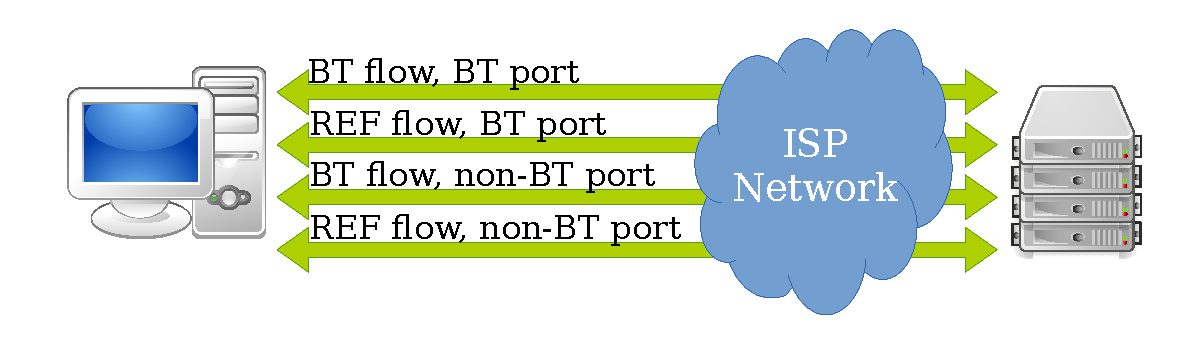
\includegraphics[width=3.3in]{figures/glasnost}
\caption{Schematic view of how glasnost works.}
\label{fig:glasnost}
\end{figure}

This measurement can be performed by logging into Glasnost test page and loading the Java\texttrademark applet. This design will not allow mobile devices to run the test as mobile devices can not run Java applets in their web browsers. Additionally, Glasnost is designed only to detect BitTorrent traffic differentiation.

\section{Methodology}
\label{sec:method}

The method used here to detect differentiation is quite similar to that of Glasnost. To see if an ISP treats a certain type of traffic differently, we first record all packets transmitted/received during a sample run of that service, replay it on the cell network using a controlled server and then repeat this process (replaying the recorded trace) on an encrypted channel. This process is repeated 5 times for each channel (encrypted and unencrypted). Finally, if the ISP treats traffic differently, metrics calculated for each channel should be significantly different (i.e. significantly more delay on 
Skype traffic when replaying on an unencrypted channel). Figure~\ref{fig:meddle} is a rough sketch of what happens during a test.

As stated before, this approach resembles that of Glasnost, meaning that it also can only detect differentiation based on port/packet payload. The reason for this is that it is not possible to send/receive recorded data to/from the original servers (e.g. Skype servers). So if the ISP differentiates based on host, it will go undetected. But ISPs usually differentiate based on port/packet payload \cite{glasnost}.

\begin{figure}[ht]
\centering
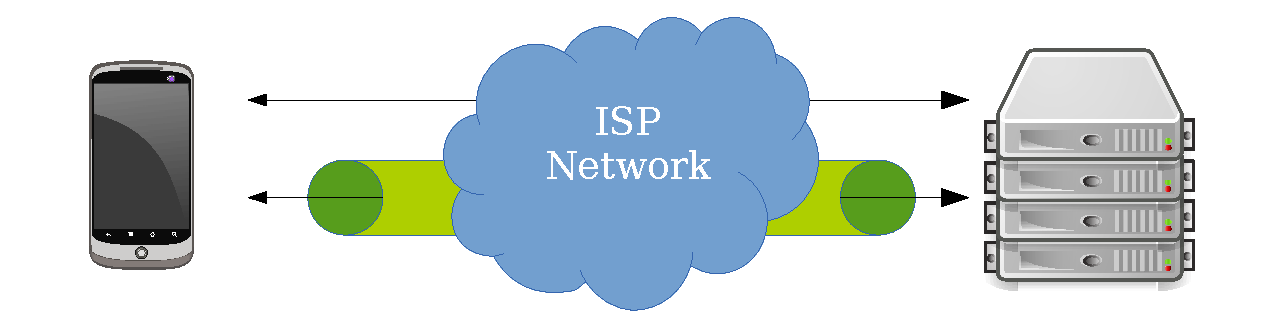
\includegraphics[width=3.5in]{figures/meddle}
\caption{Schematic view of how our project works.}
\label{fig:meddle}
\end{figure}

\subsection{Services}

A number of services were selected to test for differentiation on wireless networks. These tests each represented a category that was suspected to be differentiated by wireless providers.

For the VoIP category, Skype was chosen because it is a widely used service. For file sharing and P2P, Dropbox (upload and download) and BitTorrent were chosen respectively. Netflix, Hulu+ and YouTube (upload and download) represent video, and Spotify and Pandora represent audio in the streaming category.
\subsection{Recording Traces}

Packet traces for sample sessions for each service had to be recorded first in order to be replayed later over a cellular network. In order to do so, a mobile phone was connected to a VPN (in WiFi mode) server that recorded all of the packets in pcap format using \texttt{tcpdump}. When connected to the VPN, an action that required network interaction on the phone would be initiated and after enough data was transferred, the action would be interrupted and the VPN connection would be disconnected.

A few qualities had to be verified about reference service trace: the reference WiFi network on which the packets were recorded should be well provisioned itself (i.e. no service differentiation mechanism should be in place), so the traces were recorded on campus WiFi network. Additionally, tested applications shouldn't behave differently on WiFi compared to when they are on cellular network. This was confirmed for all tested applications by recording traces once on a WiFi network and an HSDPA+ network with roughly the same bandwidth.

\begin{figure}[ht]
\centering
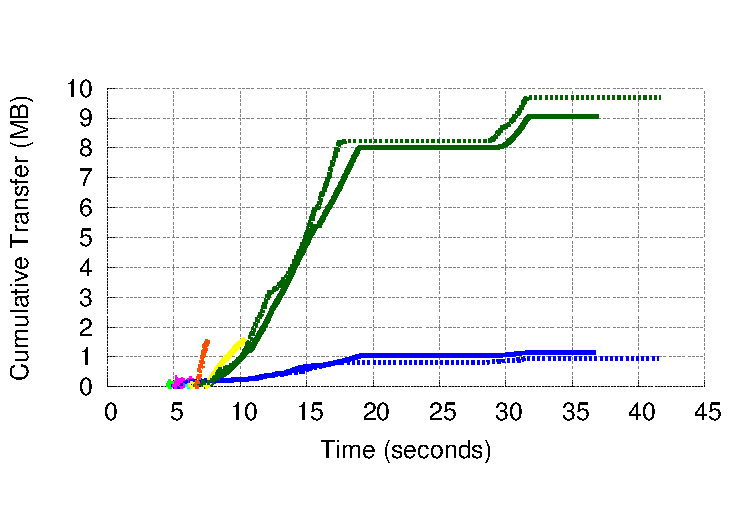
\includegraphics[width=3.3in]{figures/netflix_seqnum_wifi_vs_cell}
\caption{Sequence number plots for connections made during Netflix two sessions on WiFi (solid) and HSDPA+ (dashed) look similar.}
\label{fig:nfx_double}
\end{figure}

\subsection{Replay}

To replay the trace, a copy of the pcap file is sent to the server and a copy is kept on the client. The client will establish each connection to the server on the same port. The server will do the same and only sends packets once it has seen the packets it expects to have seen based on the pcap file it has. A pcap of this replay will be kept on the client for analysis.

For the replay we needed to decide if we wanted to preserve the inter-packet timing that would reflect application level flow control. Because the reference packet traces were recorded on a WiFi network with significantly higher bandwidth, this would have no effect on the outcome of the tests because this wouldn't affect the differentiation.

\begin{figure}[ht]
\centering
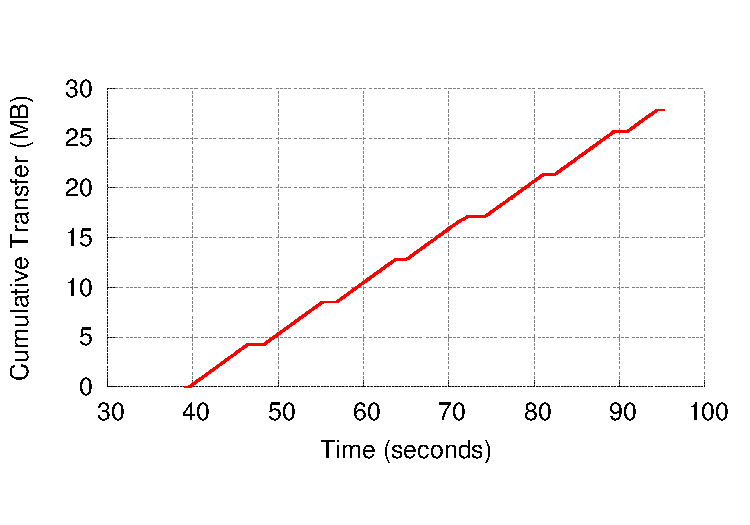
\includegraphics[width=3.3in]{figures/db_big_u}
\caption{Sequence number plot for a connection made during a Dropbox upload session on WiFi showing application-level flow control.}
\label{fig:dbu}
\end{figure}


\begin{figure}[ht]
\centering
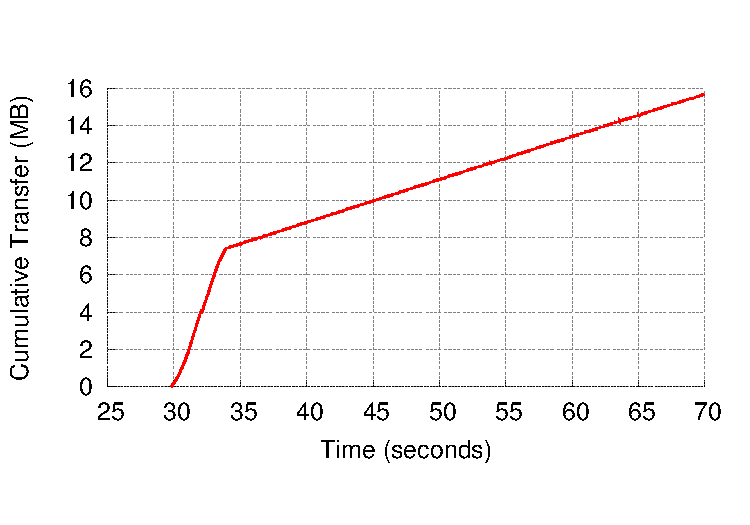
\includegraphics[width=3.3in]{figures/ytd}
\caption{Sequence number plot for a connection made during a YouTube video session on WiFi showing application-level flow control.}
\label{fig:dbu}
\end{figure}

\subsection{Noise Packets}

A smartphone that is connected to the Internet will always send and receive packets due to the services and applications that are running in the background (e.g. mail clients, update agents) so it was decided not to eliminate those packets because they were a natural part of what happens during a session.

Although for the plots, the connections shown are the ones with the largest amount of transferred bytes. If the connection's total bytes transferred during a session multiplied by a threshold is larger than or equal to the connection with largest number of bytes transferred in that session, it will be in the plot. Figure~\ref{fig:tors} demonstrates this method.

\begin{figure}[ht]
\centering
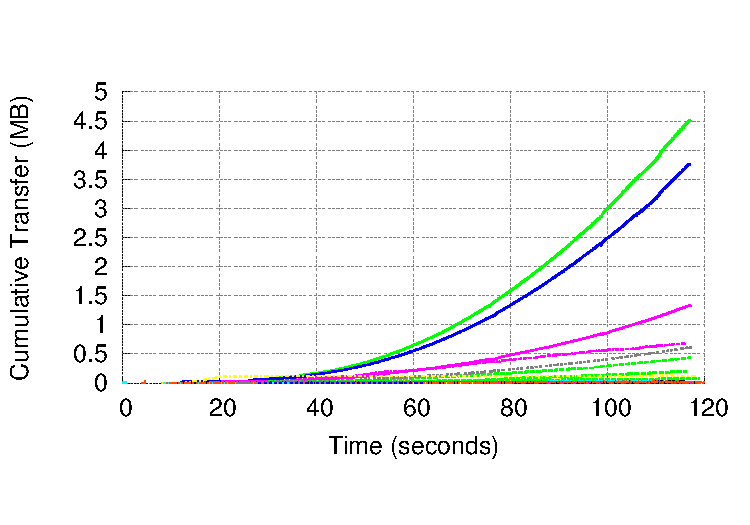
\includegraphics[width=3.3in]{figures/tor_nothr}
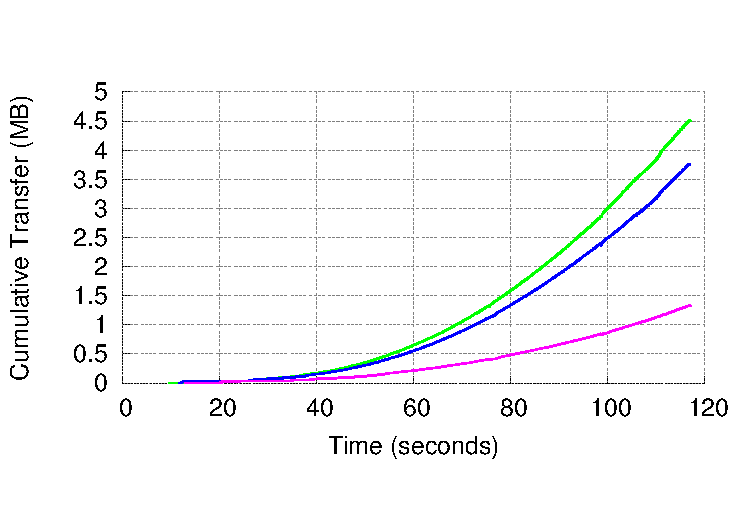
\includegraphics[width=3.3in]{figures/tor_thr}
\caption{Sequence number plot for connections made during a BitTorrent session on WiFi. Top: without a cut-off threshold, Bottom: With a cut-off threshold of 4}
\label{fig:tors}
\end{figure}

\subsection{Metrics}

Metrics that are calculated include round-trip times (RTT), throughput, and loss rate. These metrics are calculated for both channels (encrypted and unencrypted) and compared to detect differences.

In cases that there are statistically significant differences between the metrics for a service, a differentiation mechanism is suspected to exist. This can be further investigated by other methods (e.g. repeating the test). Figure~\ref{fig:att_dbu} shows an example of this.

\begin{figure}[ht]
\centering
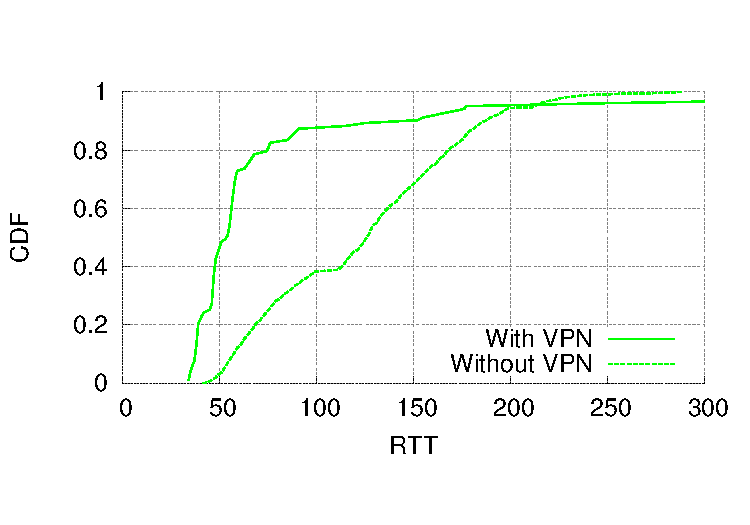
\includegraphics[width=3.3in]{figures/att_dbu_cdfrttp}
\caption{CDF for RTT samples of YouTube upload sessions on AT\&T network show higher RTTs when not encrypted.}
\label{fig:att_dbu}
\end{figure}

Note that some difference in throughput between encrypted and unencrypted replays is expected (and observed, Figure~\ref{fig:xputs}) because at the same bandwidth, a VPN connection will add overhead to the packets. Another reason for this maybe the processing carried out by the replay scripts to verify packets using hash functions.

\begin{figure}[ht]
\centering
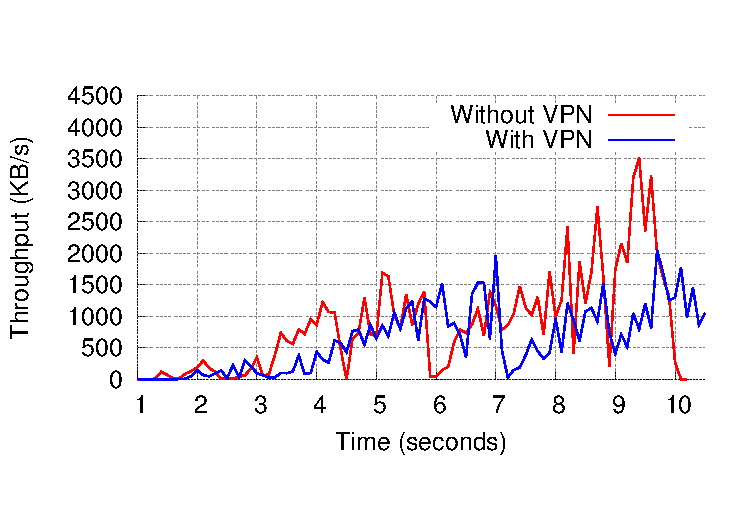
\includegraphics[width=3.3in]{figures/xp}
\caption{Throughput calculated over 0.1 second intervals for a Spotify session on AT\&T. Throughput for the VPN connection is generally lower than that of the unencrypted connection.}
\label{fig:xputs}
\end{figure}

\section{Results}

Tests were performed on a number of well-known wireless providers in north America and results indicated that differentiation mechanisms are not in fact present in those networks.

Also, as mentioned before, significantly different metrics in a network, while rising suspicion about its treatment of a certain type of traffic, will be inconclusive until complemented by further testing.

Table~\ref{tab:svcdiff} shows test results from Verizon. These results show that in fact there isn't a differentiation mechanism in their network for any of the tested services. Loss rates for all of the tests were within error margins.
\begin{table}
\centering
\begin{small}
\setlength{\tabcolsep}{.01em}
\begin{tabular}{|c|c|c|c|c|}
\hline
\multirow{2}{*}{\bf App}&\multicolumn{2}{c|}{\bf Throughput (KB/s)}& \multicolumn{2}{c|}{\bf Loss (\%)} \tabularnewline
\cline{2-5}
                             &{\bf No VPN} &{\bf VPN}&{\bf No VPN}&{\bf VPN}   \tabularnewline
                             &{\bf (avg, stdev)} &{\bf (avg, stdev)}&{\bf (avg, stdev)}&{\bf (avg, stdev)}   \tabularnewline
\hline

YT(DL)&(103.74, 31.16)&(99.85, 35)&(0.81, 0.06)&(0.86, 0.13) \tabularnewline
\hline
YT(UL)&(114.52, 6.05)&(117.37, 8.78)&(0.03, 0.01)&(0.05, 0.01) \tabularnewline
\hline
DB(DL) &(155.09, 32.42)&(148.1, 44.95)&(0.79, 0.31)&(0.88, 0.38) \tabularnewline
\hline
DB(UL)&(115.07, 7.31)&(120.25, 5.85)&(0.07, 0.02)&(0.09, 0.01) \tabularnewline
\hline
SPTFY&(123.91, 40.19)&(127.16, 45.96)&(0.83, 0.08)&(0.73, 0.07) \tabularnewline
%\hline
%PNDR&(126.01, 36)&(122.81, 28.42)&(1.08, 0.09)&(1.13, 0.10) \tabularnewline
\hline
NFLX&(122.81, 28.42)&(132.26, 33.55)&(0.97, 0.03)&(0.99, 0.15) \tabularnewline
\hline
\end{tabular}
\end{small}
\caption{ \textbf{Average and standard deviation for 4  apps } \emph{(YT: YouTube, DB: Dropbox, SPTFY: Spotify, NFLX: Netflix; UL=Upload, DL=Download) on 
Verizon. The differences in performance are within the noise, indicating no service differentiation. }}
\label{tab:svcdiff}
\end{table}

\section{Future Work}

Currently, the testing and measurement is done on a laptop tethered to a phone by a researcher. The next step would be to implement a cell phone application that does this experiment automatically so that people can freely download the app and perform measurements themselves. This way, more data will become available and the results would be more dependable for the existing cellular networks, as well as giving data to detect differentiation on newer ones.

Additionally, such platform will reveal possible differentiation variations on the same network in different regions.

%% sample bib file with references.
\begin{small}
\bibliographystyle{abbrv}%ieeetr}	
\bibliography{oni}
\end{small}


\end{document}




